\section{Result}
\label{sec:result}

\subsection{Homogeneous grid}
A homogeneous grid containing $1024$ nodes where the position of each node has been perturbed a small amount was used to execute the algorithm with several different choices of parameters, with a focus on the maintenance parameter, $\mu$. Figure \ref{fig:sources} shows the simulations for various values of $\mu$ when having many sources and only one sink in the graph. Figure \ref{fig:sinks} shows the simulations for various values of $\mu$ when having many sinks and only one source in the graph. The solutions that is found when $\mu=1$ are the shortest paths between each source and sink. When $\mu > 1$, the path chosen may not be the shortest path and there also exists a preference to share paths. Observe that the results presented are when the solution is stable, i.e. when the network pattern it creates tend not to drastically change.

\begin{figure}
\centering
\begin{subfigure}[b]{0.48\textwidth}
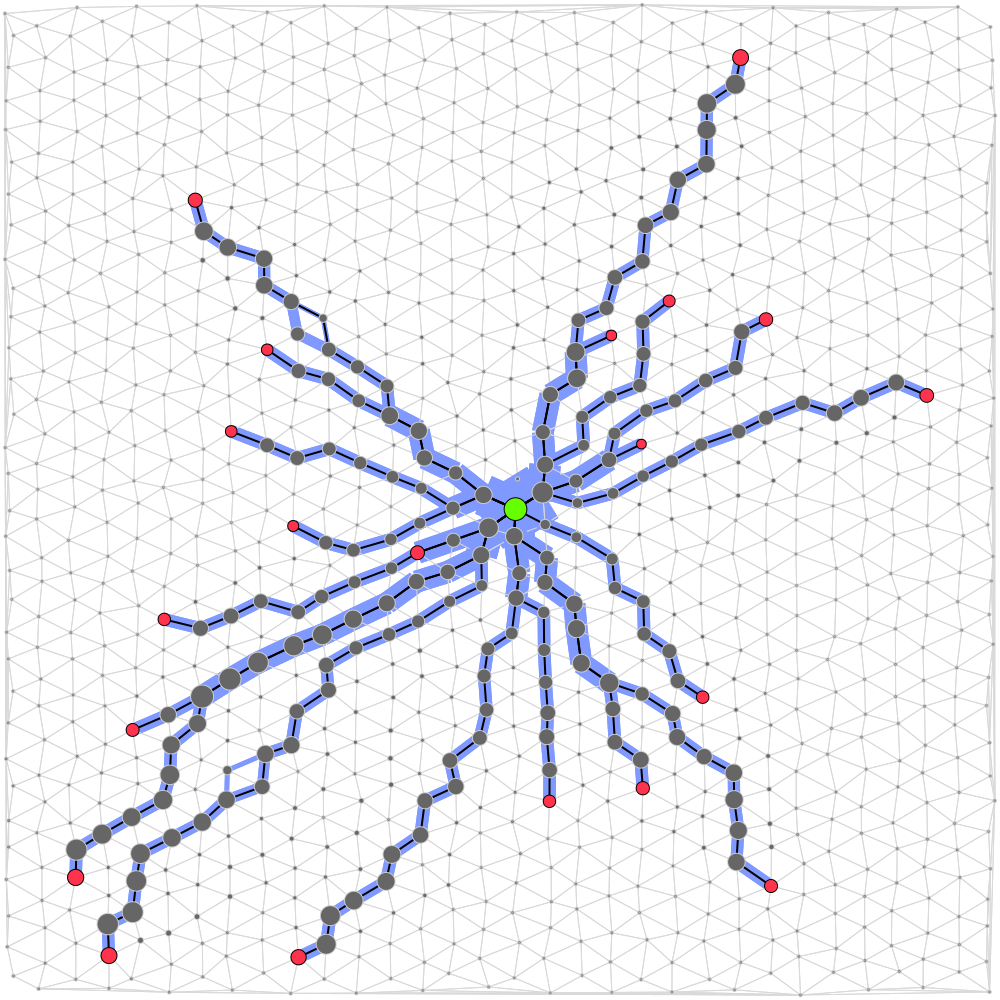
\includegraphics[width=\textwidth]{{img/nodes_sources_M10_mu1.0}.png}
\caption{The simulated solution when $\mu=1$. Solution at approximately $1400000$ time steps.}
\end{subfigure}
~
\begin{subfigure}[b]{0.48\textwidth}
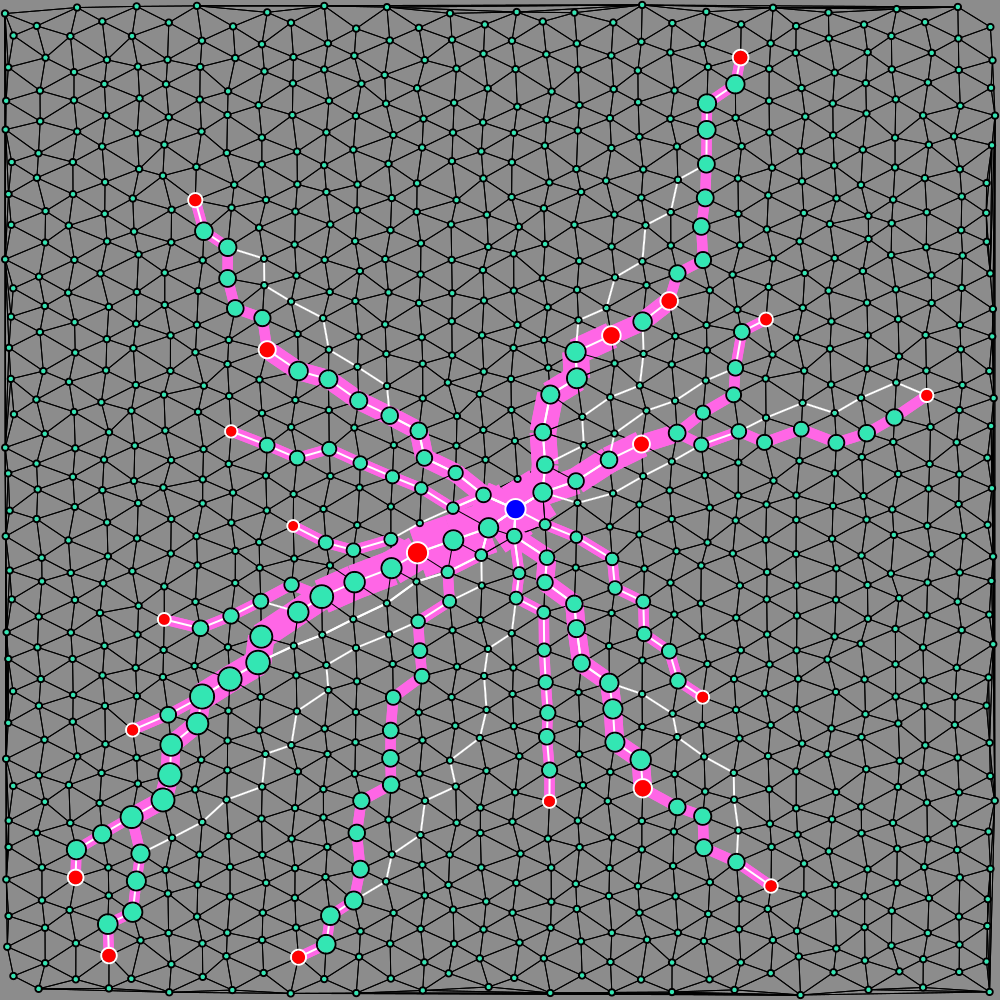
\includegraphics[width=\textwidth]{{img/nodes_sources_M10_mu1.05}.png}
\caption{The simulated solution when $\mu=1.05$. Solution at approximately $20000$ time steps.}
\end{subfigure}

\begin{subfigure}[b]{0.48\textwidth}
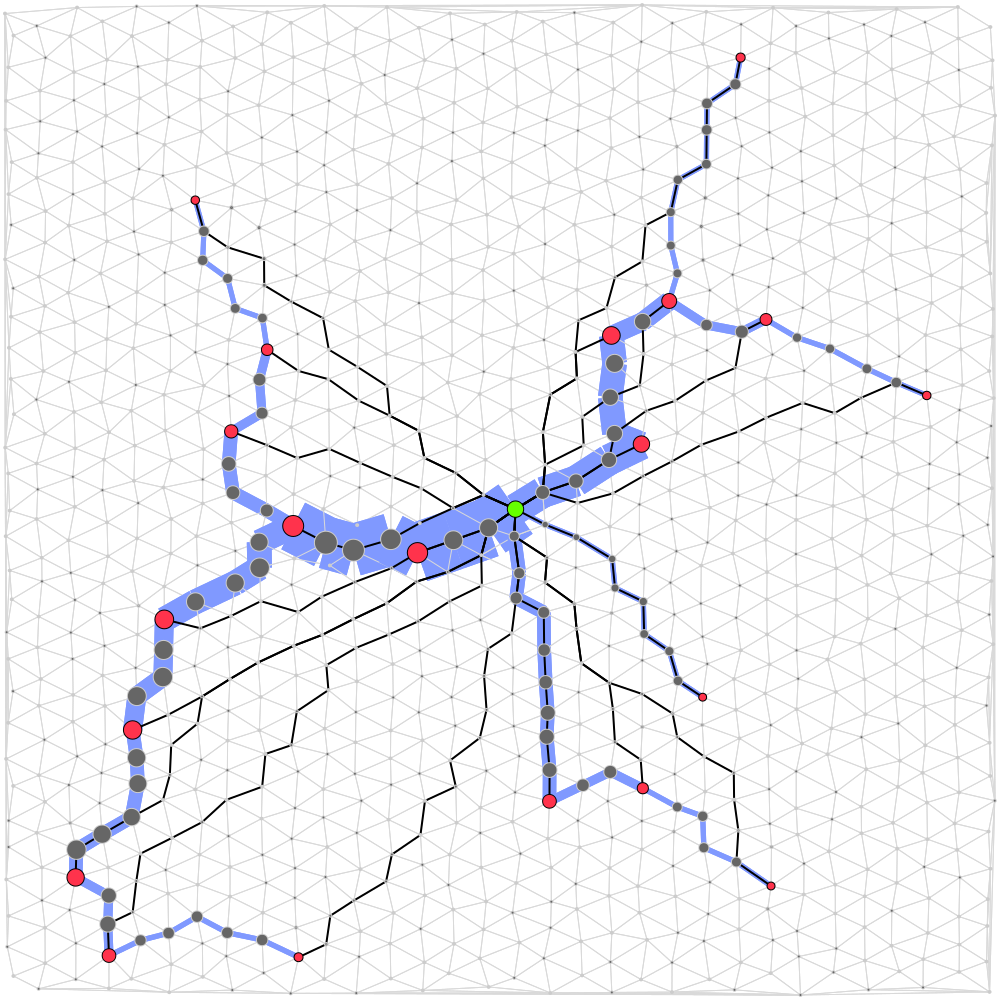
\includegraphics[width=\textwidth]{{img/nodes_sources_M10_mu1.4}.png}
\caption{The simulated solution when $\mu=1.4$. Solution at approximately $45000$ time steps.}
\end{subfigure}
~
\begin{subfigure}[b]{0.48\textwidth}
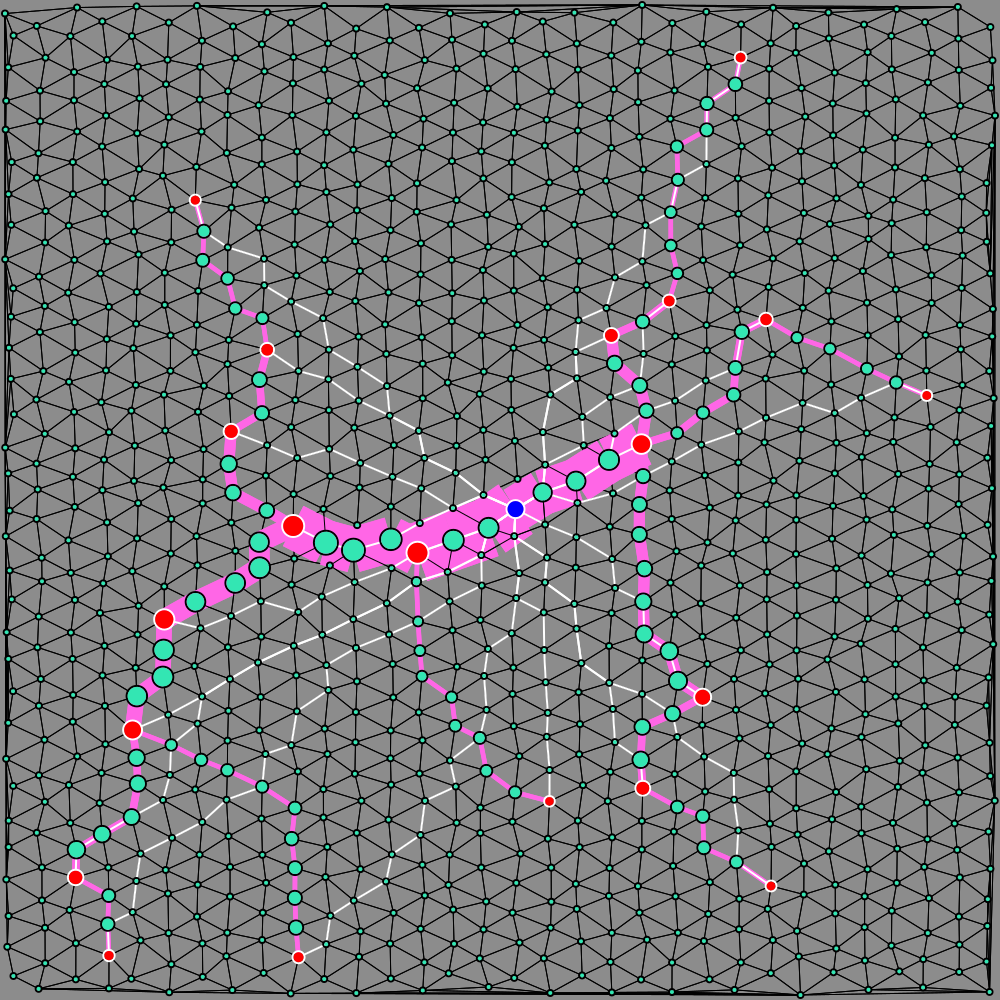
\includegraphics[width=\textwidth]{{img/nodes_sources_M10_mu1.5}.png}
\caption{The simulated solution when $\mu=1.5$. Solution at approximately $50000$ time steps.}
\end{subfigure}
\caption{Figure shows the solutions found by running the simulation on a homogeneous grid containing $1024$ nodes where the position of each node has been perturbed a small amount. The blue lines show the conductivity along each edge, where the thickness of the line is proportional to the conductivity. The shortest path found with Dijkstra's algorithm from each source to each sink has been marked with a thin black line \cite{Dijkstra}. The parameters used are $q = 10^{-4}$, $\lambda = 10^{-3},$ and $D_{min}=5 \cdot 10^{-2}$ with a time step of one. In this graph there are in total one sink and $20$ sources. Each source (red) produces 1000 particles each time unit and the sink (green) can remove as many particles as are produced each time unit.}
\label{fig:sources}
\end{figure}

\begin{figure}
\centering
\begin{subfigure}[b]{0.48\textwidth}
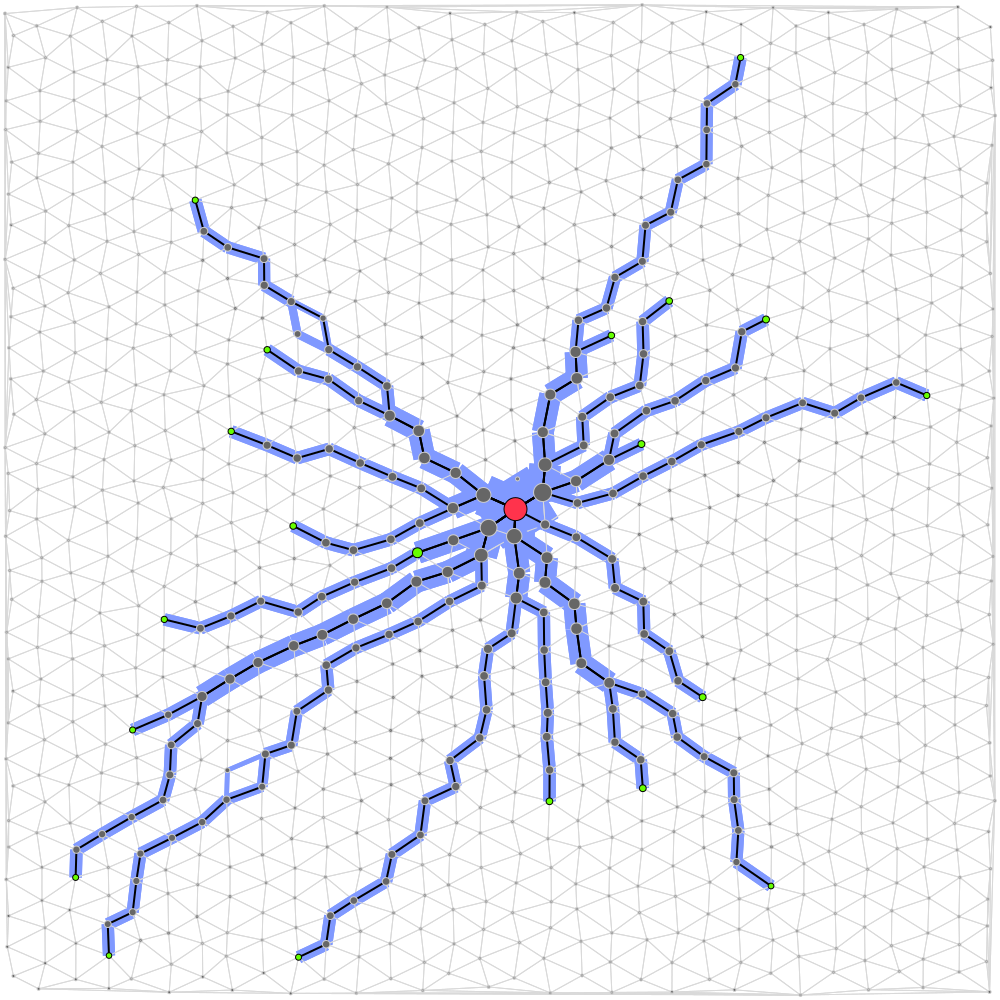
\includegraphics[width=\textwidth]{{img/nodes_sinks_M10_mu1.0}.png}
\caption{The simulated solution when $\mu=1$. Solution at approximately $1400000$ time steps.}
\end{subfigure}
~
\begin{subfigure}[b]{0.48\textwidth}
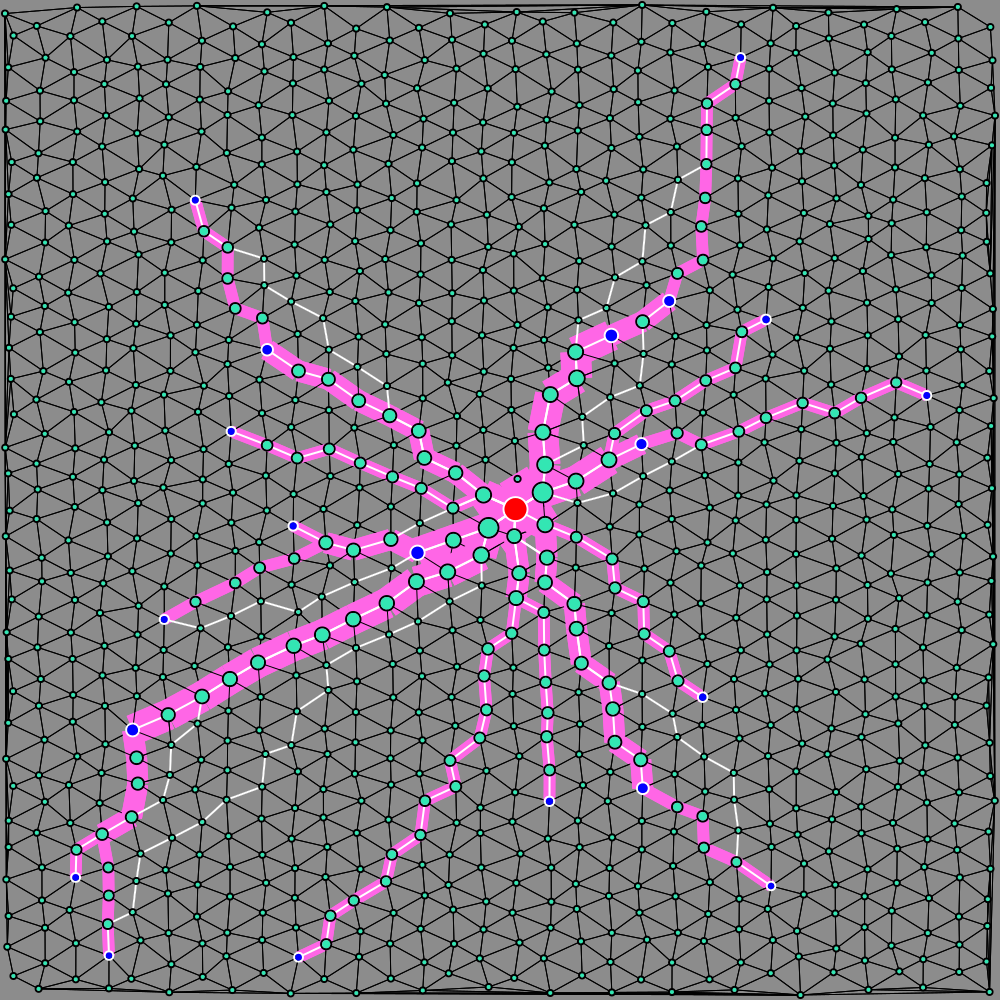
\includegraphics[width=\textwidth]{{img/nodes_sinks_M10_mu1.05}.png}
\caption{The simulated solution when $\mu=1.05$. Solution at approximately $120000$ time steps.}
\end{subfigure}

\begin{subfigure}[b]{0.48\textwidth}
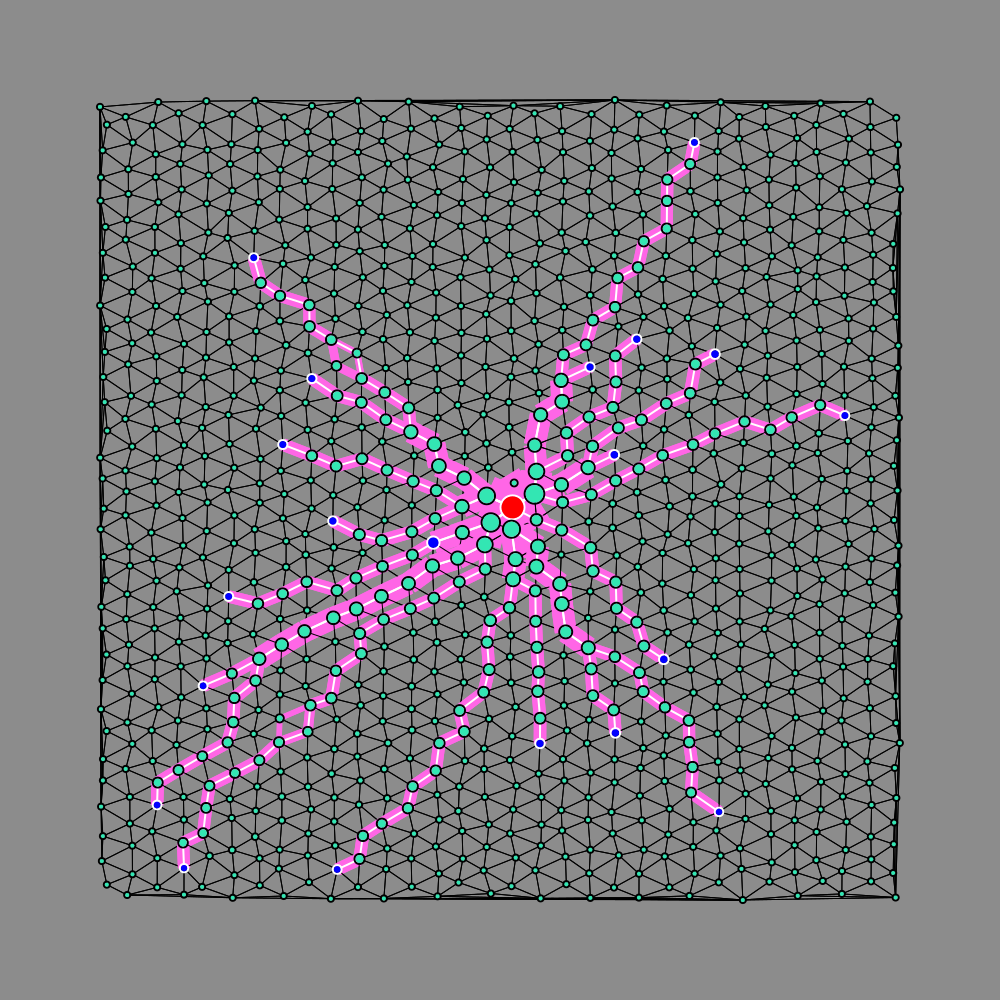
\includegraphics[width=\textwidth]{{img/nodes_sinks_M10_mu1.4}.png}
\caption{The simulated solution when $\mu=1.4$. Solution at approximately $20000$ time steps.}
\end{subfigure}
~
\begin{subfigure}[b]{0.48\textwidth}
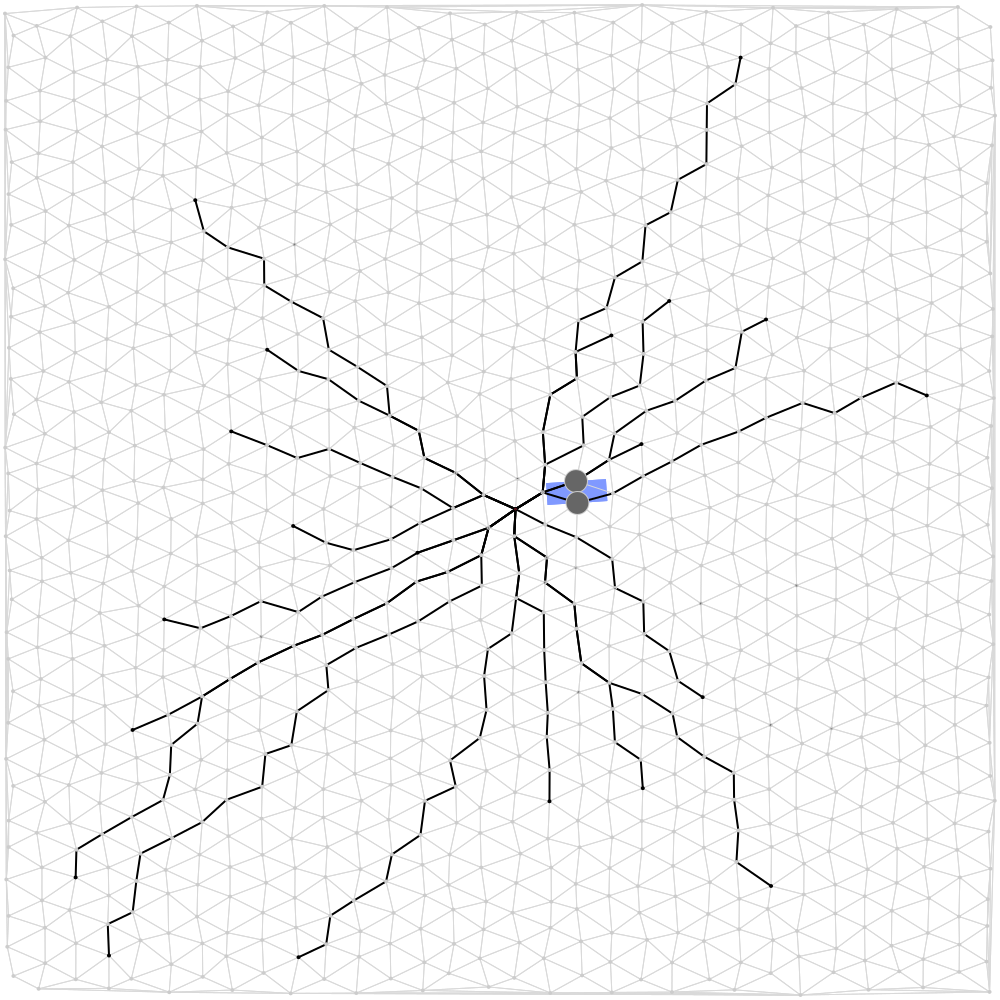
\includegraphics[width=\textwidth]{{img/nodes_sinks_M10_mu1.5}.png}
\caption{The simulated solution when $\mu=1.5$. Solution at approximately $20000$ time steps.}
\end{subfigure}
\caption{Figure shows the solutions found by running the simulation on a homogeneous grid containing $1024$ nodes where the position of each node has been perturbed a small amount. The blue lines show the conductivity along each edge, where the thickness of the line is proportional to the conductivity. The shortest path found with Dijkstra's algorithm from each source to each sink has been marked with a thin black line \cite{Dijkstra}. The parameters used are $q = 10^{-4}$, $\lambda = 10^{-3},$ and $D_{min}=5 \cdot 10^{-2}$ with a time step of one. In this graph there are in total one source and $20$ sinks. The source (red) produces 1000 particles each time unit and all sinks (green) can together remove as many particles as are produced each time unit (evenly divided between the sinks).}
\label{fig:sinks}
\end{figure}

\subsection{City}
Another graph was created using road data from OpenStreetMaps for the city of Uppsala, Sweden. Figure \ref{fig:uppsala} shows the result of the simulation when sources are placed in the residential areas and sinks are placed in the city centre. This can be seen as a simulation of traffic flow during rush hours. 

\begin{figure}
\centering
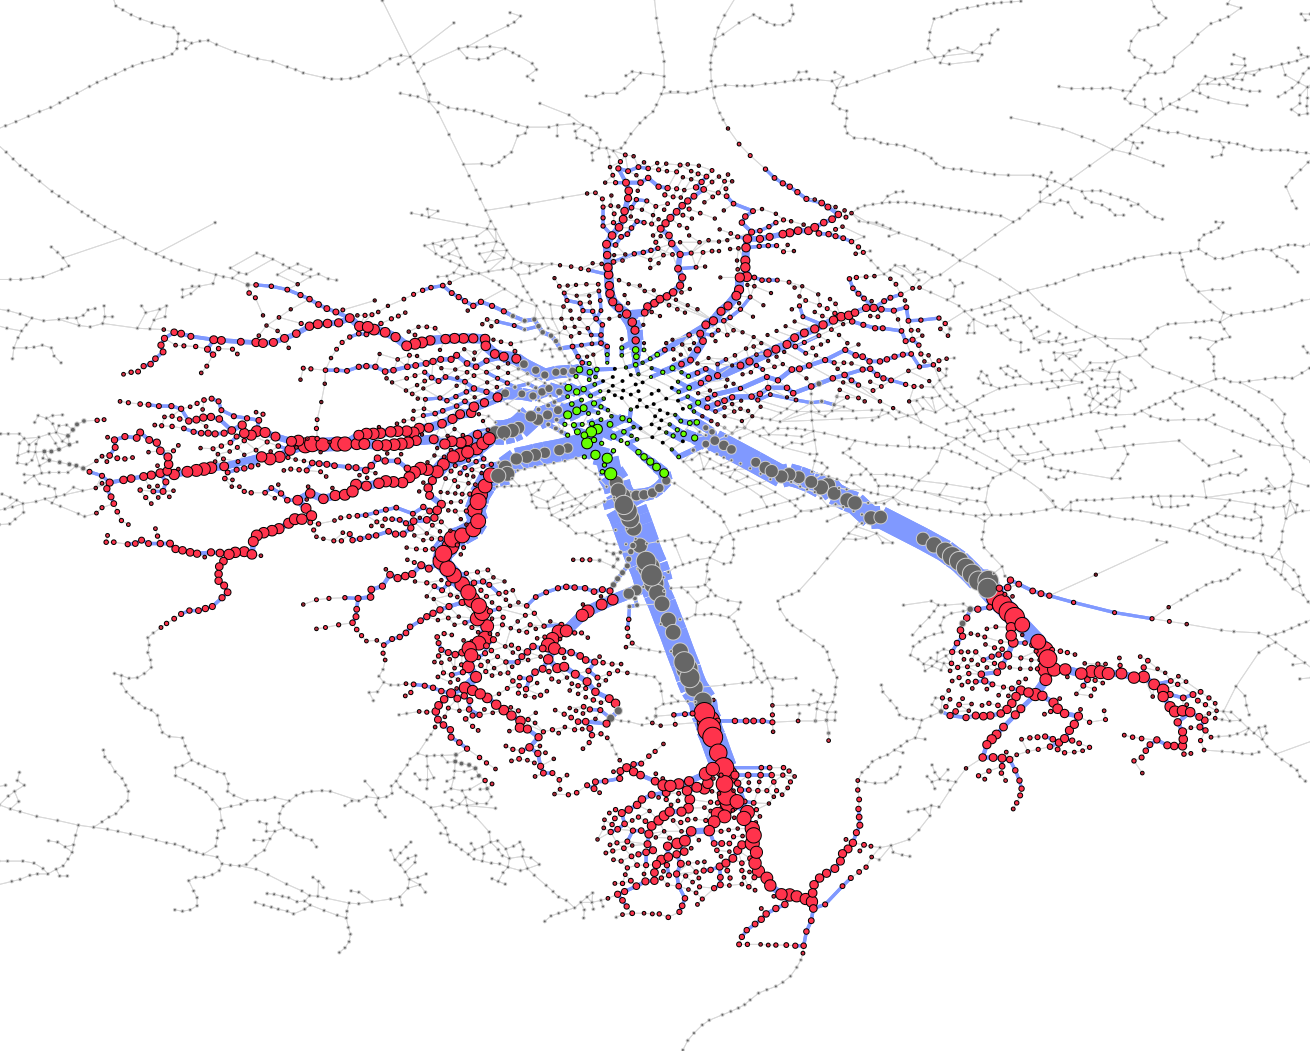
\includegraphics[width=\textwidth]{img/uppsala.png}
\caption{Figure shows the solution at $1000000$ time steps found by running the simulation on a grid of the city of Uppsala, Sweden containing $5926$ nodes. Sources (red) are placed in the residential areas and sinks (green) are placed in the city centre. The total production rate is $80000$ per time unit, equally divided between all sources. Similarly, the total removal rate is $80000$ per time unit, equally divided between all sinks. The blue lines show the conductivity along each edge, and the thickness of the line is proportional to the conductivity. The parameters used are $\mu = 1.1$, $q = 10^{-4}$, $\lambda = 10^{-3},$ and $D_{min}=5 \cdot 10^{-2}$ with a time step of $0.1$.}
\label{fig:uppsala}
\end{figure}

\subsection{Parallelism}
The measurements used to benchmark the performance of the parallel OpenMP implementation was speedup and sizeup. Figure \ref{fig:speed_size} shows the result from the speedup and sizeup measurements. All benchmarking were done on the Uppsala University servers \textit{vitsippa.it.uu.se} and \textit{tussilago.it.uu.se}, both with specifications: 

\begin{itemize}
\item CPU: AMD Opteron (Bulldozer) 6282SE, 2.6 GHz, 16-core, dual socket
\item Memory: 128 GB
\item OS: Scientific Linux 6.5.
\end{itemize}

\noindent All \texttt{C++} code was compiled with \texttt{gcc 4.8.2} with the \texttt{-fopenmp}, \texttt{-O3} and  \texttt{-static-libstdc++} flags.

\begin{figure}
\centering
\begin{subfigure}[b]{1\textwidth}
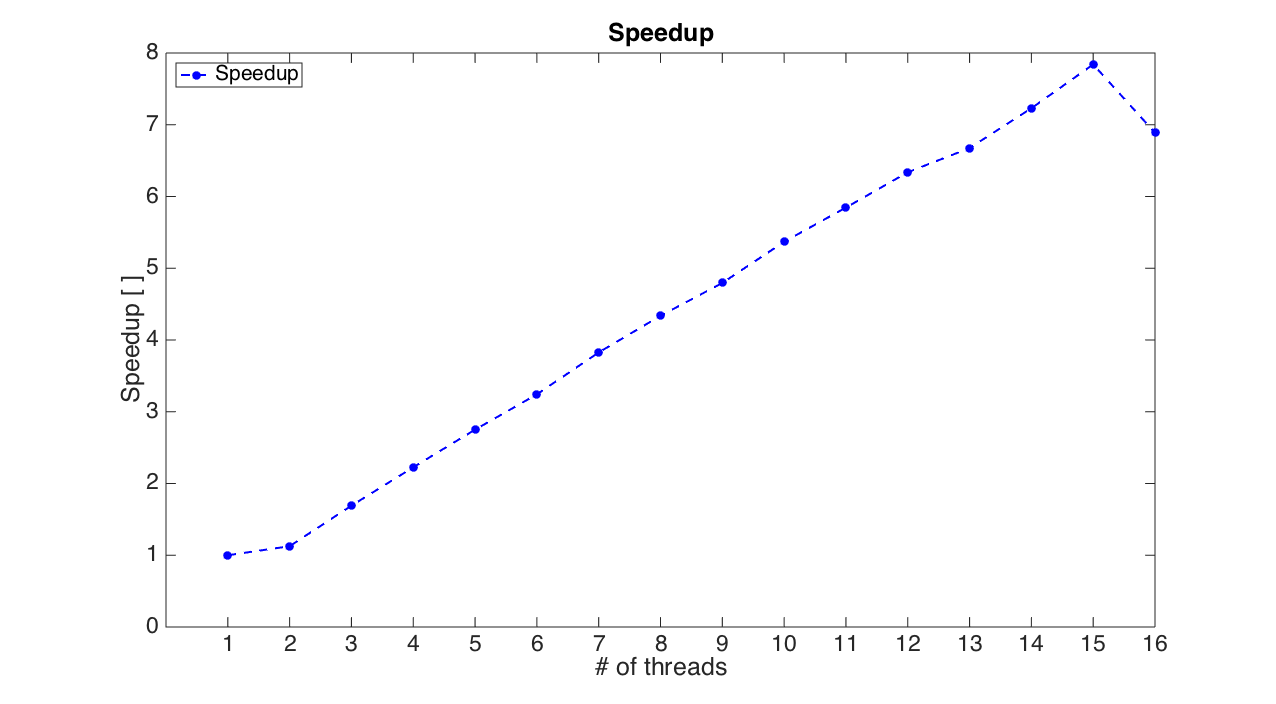
\includegraphics[width=\textwidth, height=0.5\textwidth]{img/speedup.png}
\caption{The speedup of the parallel implementation. A uniformly randomized grid containing $10000$ nodes was used for measuring the speedup. The simulation was run for $1000$ iterations with a time step of $0.1$.}
\end{subfigure}

\begin{subfigure}[b]{1\textwidth}
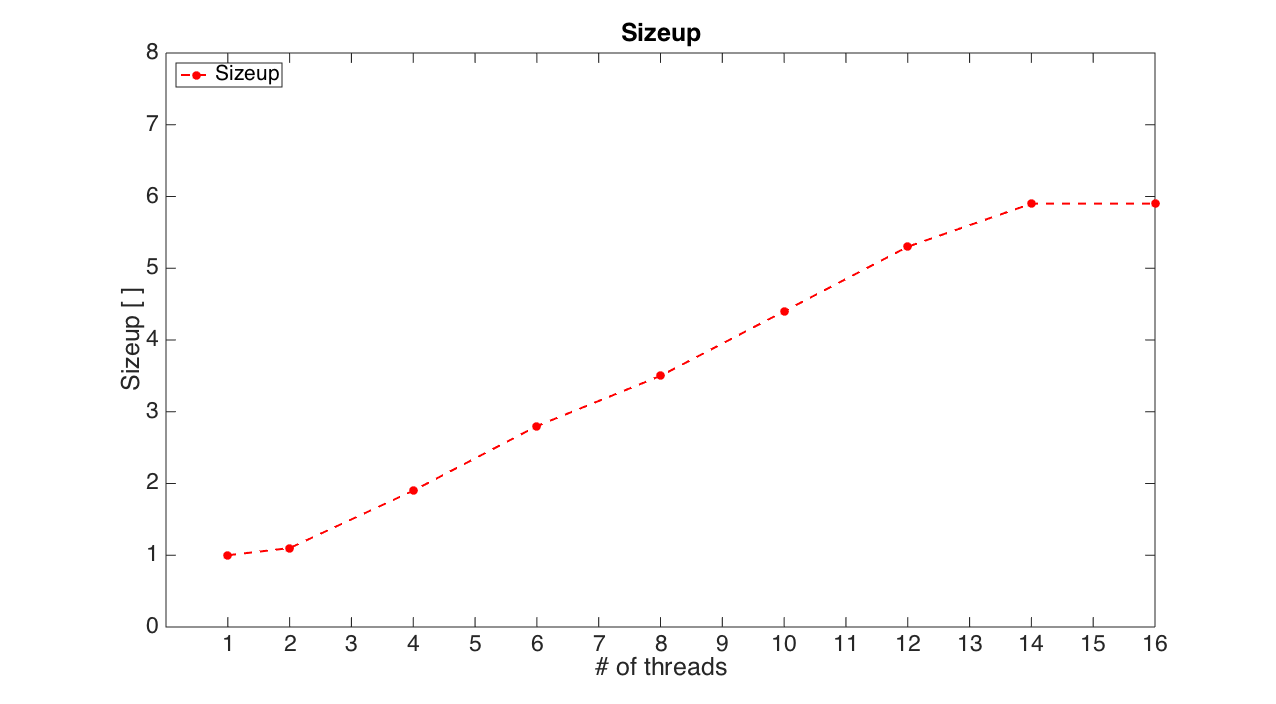
\includegraphics[width=\textwidth, height=0.5\textwidth]{img/sizeup.png}
\caption{The sizeup of the parallel implementation. The reference size, i.e. the size of the problem when sizeup is one was a uniformly randomized grid containing $5000$ nodes. The computation time used for measuring the sizeup was $60~s$ with an allowed variation of $\pm 3~s$. }
\end{subfigure}
\caption{Figure shows the different measurements of the parallel implementation of the algorithm presented in Algorithm \ref{alg:outline}. All benchmarking was run three times per data point and the best performance among those data points was extracted and used in these results.}
\label{fig:speed_size}
\end{figure}

